\section{Sensor}
Sensoren som bliver beskrevet i hardware afsnittet skal kommunikere med arduino boardet. Dette kræver nogle trin som kan findes i databladet til sensoren. På figur \ref{sensor_kom} ses et overblik over funktioner der skal til for at aflæse sensoren. Disse funktioner vil blive uddybet i dette afsnit.

\begin{figure}[h!]
  \centering
  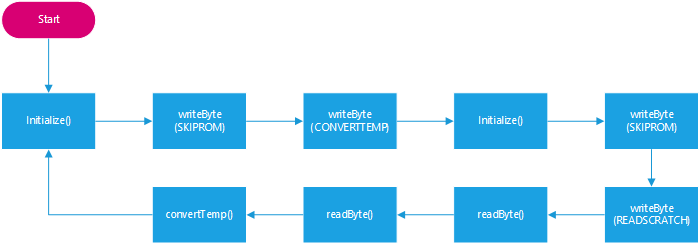
\includegraphics[width=0.8\textwidth]{figures/ds18b20_sensor_communication.png}
  \caption{Kommunikation med sensor.}
  \label{sensor_kom}
\end{figure}
\fxnote{ret størrelse til på alle billeder(noget der skal gøres til sidst!)}


\subsection{Initialize}
Initialisering af sensoren gøres ved at sætte 1-wire forbindelsen til sensorsen til low i et specifikt stykke tid.

\begin{figure}[h!]
  \centering
  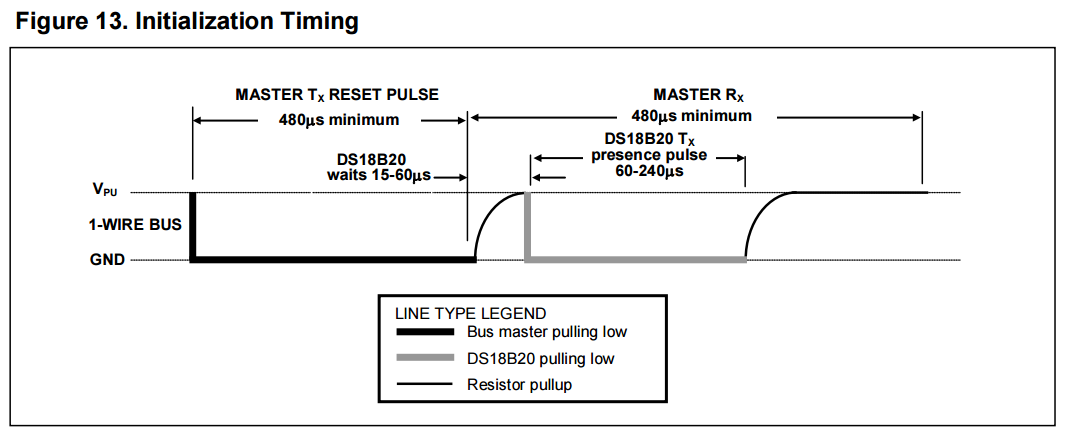
\includegraphics[width=0.5\textwidth]{figures/Initialization_timing.png}
  \caption{Fra datablad om hvordan sensor skal initialiseres.}
  \label{sensor_kom}
\end{figure}

Fra databladet ses det at 1-wire forbindelsen skal sættes til low i minimum 480$\mu$S